% declarar nenhum cabeçalho

\section{Transporte}
\subsection{Voltar para casa}

Para os calouros de fora de Campinas, além de escolher a nova morada é
importante recolher informações sobre como realizar o trajeto entre sua cidade e
Campinas.

A forma usual é ir de ônibus, mas tenha em mente que a rodoviária é longe e os
trajetos de ônibus até lá são demorados. O endereço da rodoviária é: Rua Pereira 
Lima, s/n. Há duas linhas que passam por lá: o 332 (que passa dentro da
Unicamp) para dentro da rodoviária, mas demora mais pra chegar que o 331, que
sai do terminal e para do lado de fora da rodoviária. Em horários de pico, o
trajeto pode demorar quase uma hora, então cuidado para não perder o horário do
ônibus para sua cidade. Também não se esqueça de portar algum cartão para 
andar nos ônibus de Campinas, seja o Bilhete Único ou um dos dois cartões avulsos
(Bilhete 1 Viagem e Bilhete 2 Viagens). Caso contrário, não será possível embarcar 
em um ônibus.

Os que vêm de mais longe certamente farão uso do aeroporto de Viracopos, cujo
telefone é 3725-5000. Para chegar ao aeroporto existe a linha 193 que sai da
rodoviária e vai para o aeroporto, e também faz o trajeto de volta. Porém, ir com
ônibus circular pode ser um transtorno quando estiver com mala grande. Uma outra
alternativa é a Lirabus que também faz o traslado da rodoviária para o
aeroporto. A passagem da Lirabus custa R\$9,00 (R\$9,80 se sair da Rodoviária,
pois paga taxa de embarque) e os horários podem ser conferidos no site
\url{www.lirabus.com.br/}.

Para quem for usar os aeroportos da Grande São Paulo (Congonhas e Guarulhos),
existem os serviços de traslado, também oferecidos pela Lirabus. A tarifa para
Guarulhos sai R\$28,30 (R\$33,70 com taxa de embarque da Rodoviária), e para 
Congonhas sai R\$24,45 (R\$29,90 com taxa de embarque da Rodoviária).

Para não pagar a taxa de embarque nos traslados da Lirabus, basta embarcar 
na Sala VIP da Lirabus, localizada na Avenida Francisco Glicério, 435,
em frente ao Largo do Pará.

\subsubsection*{Caronas}

Uma forma barata e divertida de viajar, além de minimizar o tempo e dinheiro
gastos na viagem, é juntando alguns estudantes no mesmo carro e dividir as
despesas.
\begin{figure}[h!]
    \centering
    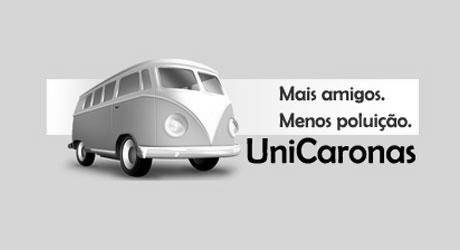
\includegraphics[width=.45\textwidth]{img/barao/unicaronas.jpg}
\end{figure}

O site UniCaronas (\url{unicaronas.com.br}) foi desenvolvido por dois
engenheiros de computação da Unicamp, com o intuito de facilitar o deslocamento
dos alunos entre cidades. Criado em 2007 como Caronas Unicamp e disponível
apenas para alunos da Unicamp, O site chegou a possuir mais de 20 mil usuários e
mediar caronas entre alunos de diversas universidades para várias cidades de
vários estados. Em 2014, o site se uniu ao Tripda (\url{tripda.com.br}),
aumentando imensamente a quantidade de destinos, mas mantendo as funcionalidades
básicas. No entanto, o site serve apenas para colocar os motoristas e caronistas
em contato, não assumindo responsabilidades sobre nenhuma das partes.

\subsection{Carro}

Para aqueles que tenham seu próprio veículo, é bom saber que a Unicamp tem
poucas vagas próximas aos locais de aulas. E o número de fiscais de trânsito tem
aumentado muito dentro do Campus.

\subsubsection*{Autoescolas}

Se você ainda não tem CNH e pretende obtê-la em Campinas, existem três opções de
autoescola em Barão Geraldo:

\begin{itemize}
    \item  \textbf{Auto Escola Avenida}
        \\Endereço: Av. Albino J. B. De Oliveira, 658
        \\Telefone: (19) 3288-0588

    \item  \textbf{Auto Escola Advanced}
        \\Endereço: Av. Santa Isabel, 80
        \\Telefone: (19) 3289-9499

    \item  \textbf{Auto Escola Mario Trentin}
        \\Endereço: Av. Santa Isabel, 513
        \\Telefone: (19) 3388-0513 / (19) 3289-2614
\end{itemize}

\subsubsection*{Recorrer de Multas}

Documentos:
\begin{itemize}
    \item  Notificação e Fotocopia.
    \item  CNH e Fotocopia.
    \item  Documento do Carro e Fotocopia.
    \item  Formulário: \url{www.emdec.com.br/eficiente/repositorio/EMDEC_documentos/5079.pdf}.
    \item  e anexos, se desejar.
\end{itemize}

E levá-los a:
\begin{itemize}
    \item   \textbf{EMDEC}
        \\Horário: De segunda a sexta-feira, das 8h as 17h.
        \\Endereço: Rua Dr. Salles Oliveira, 1028 -- Vila Industrial -- CEP 13035-270.
    \item   \textbf{Poupatempo (Centro)}
        \\Horário: Das 8h às 18h, de segunda a sexta-feira; e aos sábados, das 7h às 13h.
        \\Endereço: Av. Francisco Glicério, 935.
    \item   \textbf{Poupatempo (Campinas Shopping)}
        \\Horário: Das 9h às 19h, de segunda a sexta-feira; e aos sábados, das 8h às 14h.
        \\Endereço: Rua Jacy Teixeira de Camargo, 940.
\end{itemize}

Fonte: \url{www.emdec.com.br/eficiente/sites/portalemdec/pt-br/site.php?secao=multas&pub=31}

\subsection{Ciclovias e ciclofaixas}

Campinas possui cerca de 27 quilômetros de ciclovias e de ciclofaixas. Algumas dessas vias para 
bicicletas estão no distrito de Barão Geraldo. Uma delas é a ciclovia que liga o campus da Unicamp 
a Av. Albino J. B. de Oliveira. A outra é a ciclofaixa que liga a Av. Albino J. B. de Oliveira 
à moradia (Av. Santa Isabel).

Nos domingos e feriados, das 7 até as 12 horas, as ciclofaixas ficam abertas para os ciclistas.

\subsection{Ônibus}

Se não tem condução própria, ou carona, pode utilizar o transporte coletivo de
Campinas.

\begin{figure}[h!]
    \centering
    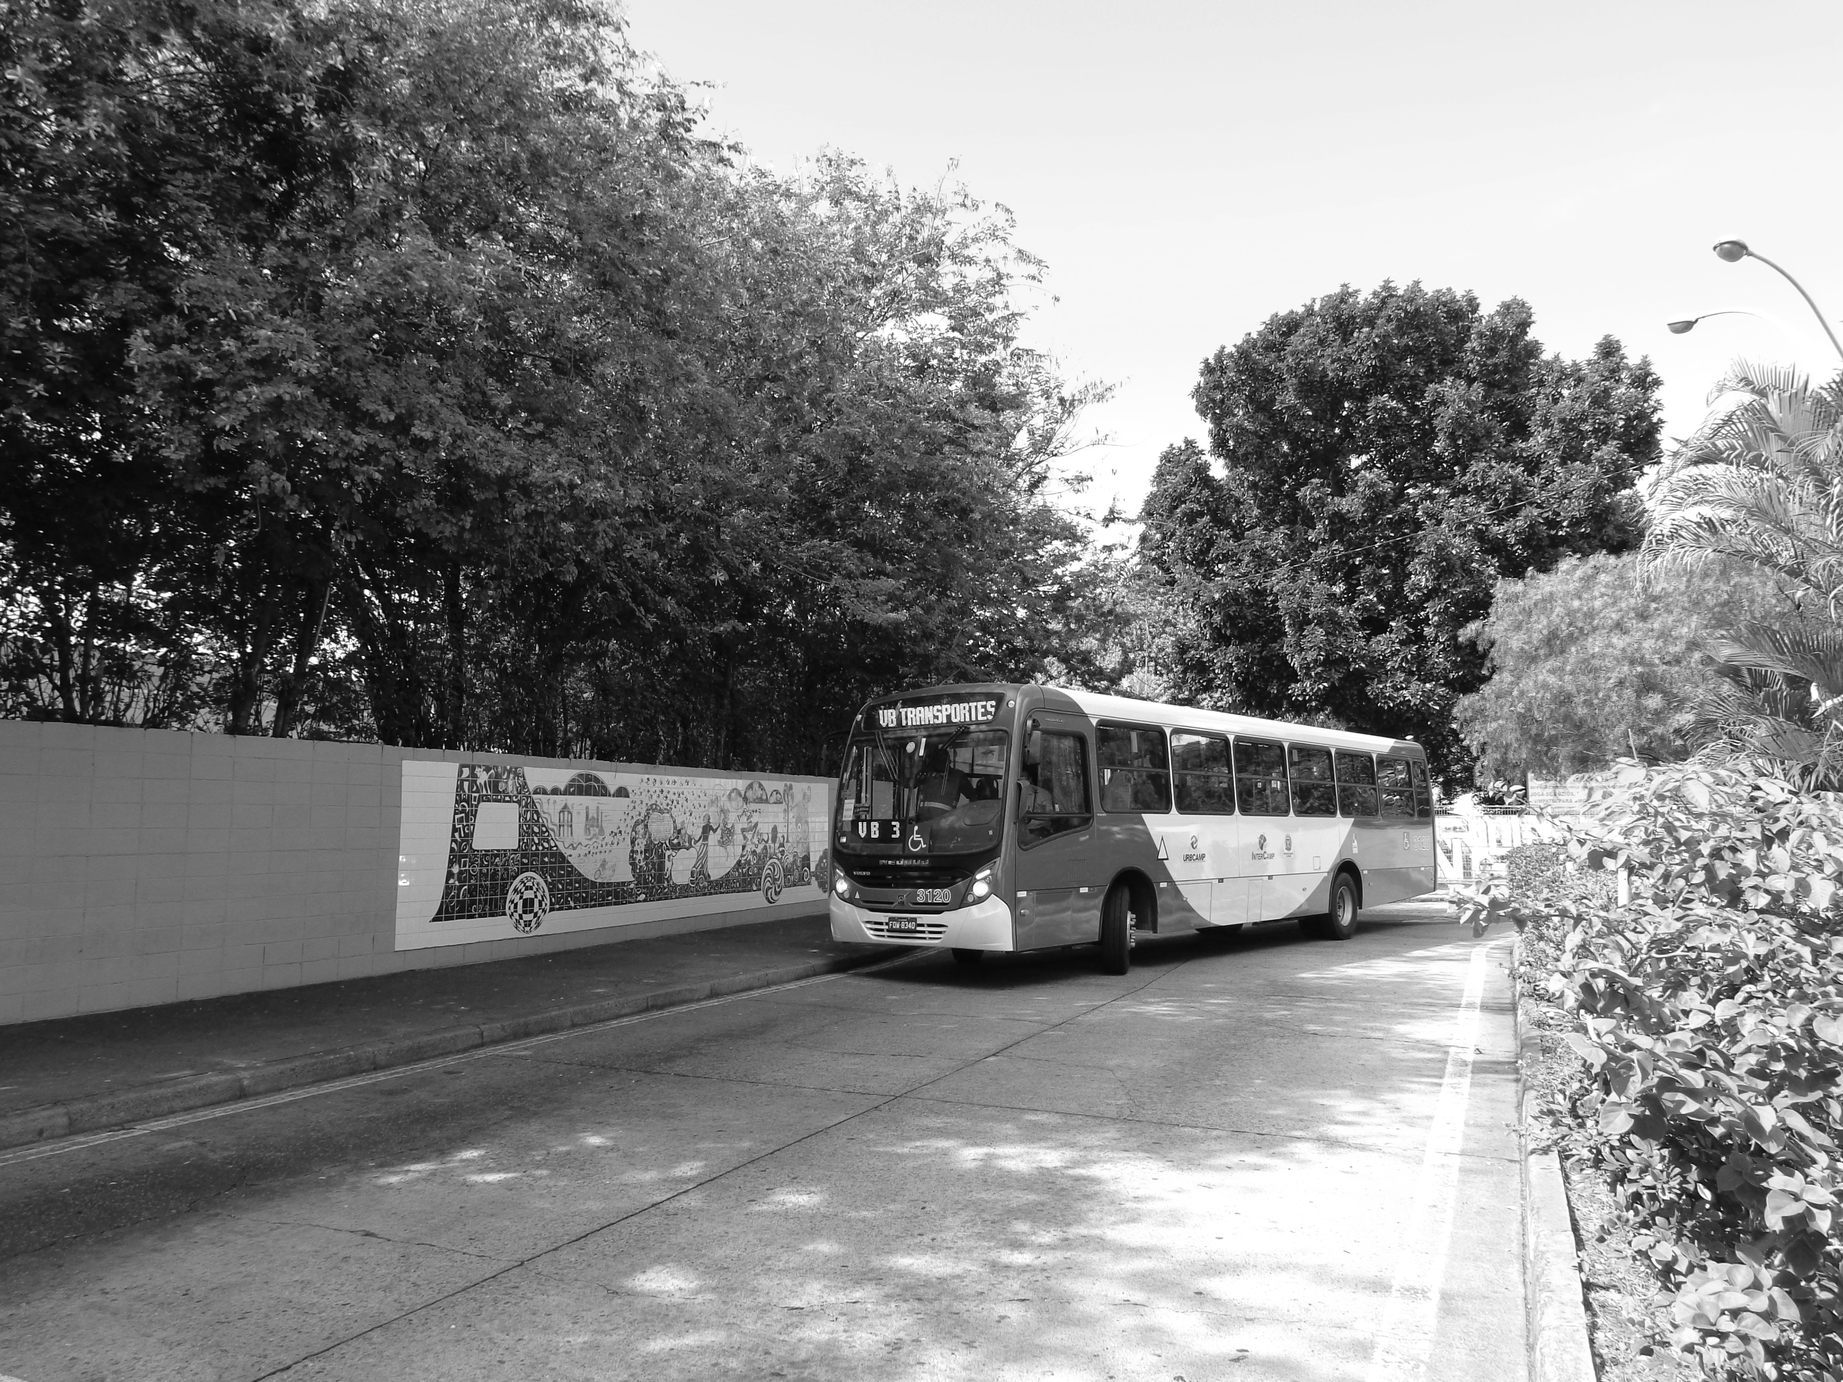
\includegraphics[width=.45\textwidth]{img/barao/onibus.jpg}
\end{figure}

O sistema de transporte público em Campinas é composto apenas por ônibus, e
chama-se InterCamp. O órgão municipal que organiza, gerencia e fiscaliza o
transporte público é a EMDEC (Empresa Municipal de Desenvolvimento de Campinas).
A bilhetagem eletrônica é organizada pela Transurc, a associação das empresas
de ônibus do transporte coletivo urbano de Campinas. Além das empresas, operam
no InterCamp cooperativas de transporte, originadas dos antigos perueiros.

Os ônibus em Campinas são identificados por um número de três dígitos, uma cor
(azul claro, azul escuro, vermelho ou verde), uma figura geométrica (círculo,
quadrado, triângulo ou tetragrama, para que os portadores de daltonismo possam
identificar os ônibus) e um nome. A tarifa foi reajustada em junho de 2013 e
custa R\$3,30. Apesar de existir passe de estudante, universitários não têm
direito ao desconto, apenas estudantes de ensino fundamental e médio. 
Entretanto, a situação está prestes a mudar, pois existe um projeto de lei
para que os universitários tenham desconto de 50\% na passagem.

Todo mês, em dois domingos, os usuários do transporte público de Campinas podem usar
os ônibus pagando metade da tarifa (o que dá R\$ 1,65). É o Passe Lazer. O benefício
vale apenas para os cartões avulsos e para o Bilhete Único Comum.

Existe quatorze linhas de ônibus que ligam o centro, alguns distritos, bairros e
terminais de Campinas ao distrito de Barão Geraldo. Algumas linhas desembarcam
os passageiros no terminal de Barão Geraldo, de onde seguem em outros ônibus
para a universidade. Já outras linhas vão direto para o campus. As trocas de
ônibus dentro do Terminal de Barão Geraldo são gratuitas, o que não ocorre em
outros terminais (no Terminal Mercado, por exemplo).

Em 2008 foi construída a nova e moderna rodoviária de Campinas, o terminal
multimodal Ramos de Azevedo. Além de transporte interestadual e municipal, o
espaço agrega um terminal metropolitano com o intuito de ligar as cidades da
Região Metropilitana de Campinas. Algumas linhas de ônibus internos de Campinas
também passam neste Terminal, como a linha 332.

Para consultar linhas de ônibus, há duas opções:
\begin{itemize}
  \item o sistema da EMDEC, que também possui um roteirizador bastante
  interessante (\url{www.emdec.com.br/ABusInf/})
  \item o site Ônibus de Campinas, do Portal InterBuss, criado por entusiastas
  de ônibus, dentre eles, um veterano da Computação 
  (\url{www.portalinterbuss.com.br/campinas/})\ldots
\end{itemize}

Outra ferramenta interessante para quem pretende usar o transporte público em
Campinas é o app Moovit, disponível para iOS, Android e Windows Phone. Com
ele, é possível visualizar os pontos de ônibus ao seu redor e as linhas que
passam neles. Além disso, também funciona como roteirizador, indicando
as linhas que você pode pegar para chegar a um lugar da cidade.

Para reclamações do transporte público, é necessário utilizar o canal 156
da Prefeitura de Campinas. Ele pode ser acessado através do telefone 156,
através do site da Prefeitura 
(\url{www.campinas.sp.gov.br/servico-ao-cidadao/156.php}), e através do 
aplicativo 156 Mobile Campinas, disponível para Android. As reclamações 
são respondidas pelos órgãos de fiscalização da EMDEC, e todo o processo pode 
levar até seis meses. Entretanto, é o único meio que pode resultar em 
ações efetivas, como multas e advertências. Além disso, a reclamação 
entra nas estatísticas da EMDEC, que são utilizadas para direcionar agentes 
de fiscalização e, caso haja algum problema operacional de itinerário ou 
de horário, também podem ser feitas alterações para otimização do serviço.

\subsubsection*{Bilhete Único}

O Bilhete Único foi implantado com o objetivo de facilitar o transporte daqueles
que se utilizam de ônibus. No prazo de 2 horas, o usuário pode usar até três ônibus 
pagando apenas uma passagem. Além disso, agora o usuário tem dois créditos negativos 
para utilizar caso o saldo seja zerado. O cadastro é rápido e o cartão sai na hora.

O Bilhete Único Comum pode ser feito nos seguintes locais:
\begin{itemize}
  \item sede da Transurc, na Rua Onze de Agosto, 757
  \item nos terminais de ônibus (guichês da Transurc, sempre próximos à entrada)
  \item na Loja do Bilhete Único, na Av. Anchieta, 55
  \item no posto da Transurc do Poupatempo Centro (Av. Francisco Glicério, 935, térreo)
  \item na Drogaria Sidarta do Balão do Londres (Av. John Boyd Dunlop) \ldots
\end{itemize}

Para a primeira recarga, exige-se o pagamento de uma tarifa (o que atualmente 
fica em R\$ 3,30).

Para recarregar o cartão, além dos terminais, também tem diversos
estabelecimentos comerciais credenciados a fazer a recarga do cartão, que podem
ser vistos na página: \url{www.transurc.com.br/site/index.php/informacoes/onde-comprar/}.

\subsubsection*{Como embarcar sem Bilhete Único}

Campinas vem extinguindo a função do cobrador, substituindo-o pela bilhetagem 
eletrônica. Várias linhas já rodam sem cobrador, e provavelmente muitos lerão 
este texto quando já estiverem completamente extintos do sistema.

A partir de 1º de fevereiro de 2015, o pagamento não poderá mais ser feito 
em dinheiro dentro dos ônibus. Com isso, os usuários deverão entrar nos veículos 
portando o Bilhete Único (vide sub-seção acima para mais informações) ou um 
cartão avulso, chamado Bilhete Viagem.

São dois Bilhetes Viagem: o Bilhete 1 Viagem e o Bilhete 2 Viagens.

O Bilhete 1 Viagem é adquirido pelo valor de R\$ 5,30, e pode ser usado apenas 
uma vez, pois não dá direito a integração. Também não pode ser recarregado. 
Por isso, é ideal apenas para quem for utilizar ônibus uma única vez.

O Bilhete 2 Viagens é adquirido pelo valor de R\$ 8,60, pode ser usado por duas 
vezes, e depois ainda pode ser recarregado em qualquer posto de recarga do 
Bilhete Único. É o cartão ideal para quem pretende utilizar ônibus mais de uma vez,
mas não pretende fazer o Bilhete Único.

Os R\$ 2,00 acima da tarifa vigente pagos na aquisição de ambos os Bilhetes Viagem 
se referem ao custo de casco do cartão, que são devolvidos ao usuário se ele 
entregar o cartão vazio em um dos postos da Transurc (sede da Transurc, terminais, 
Loja do Bilhete Único ou posto da Transurc do Poupatempo Centro).

Ambos os Bilhetes Viagem podem ser adquiridos nos postos da Transurc ou na 
rede credenciada (\url{www.transurc.com.br/site/index.php/informacoes/onde-comprar/}).
